\documentclass[12pt]{IEEEtran}
\usepackage[brazilian]{babel}
\usepackage[utf8]{inputenc}
\usepackage{amsmath}
\usepackage{mathtools}
\usepackage{indentfirst}
\usepackage{graphicx}
\usepackage{float}
\usepackage{booktabs}
\usepackage{tabularx}


\title{Relatório Experimental 2 - Prática de Física dos Dispositivos Eletrônicos}
\author{Felipe Rodrigues Sobrinho (17/0141764)}
\date{14/06/2022}


\begin{document}

\maketitle

\section{Introdução}

A lâmpada elétrica forma um dos maiores avanços tecnológicos do início do século XX. A primeira lâmpada, inventada por Thomas Edison, era constituída principalmente por um filamento de bambu carbonizado inserido dentro de um bulbo em condições de vácuo ou quase vácuo, mas com um gás inerte. 

O modelo de lâmpada incandescente ainda possuí o mesmo formato, mas agora o filamento utiliza o tugstênio como material de base.



\section{Metodologia}

Para tal experimento, foi utilizado a bancada experimental vista na figura \ref{fig:bancada}. Foi utilizado um multímetro do modelo DT9205A e uma fonte de bancada do modelo POL-16E.

\begin{figure}[H]
  \centering
  
\includegraphics[width=.48\textwidth]{bancada_imagem.png}
  \caption{Bancada experimental utilizada. A) Fonte de alimentação POL-16E; B) Multímetro DT9205A para medição de $V_A$; C) Multímetro DT9205A para medição de $V_B$; D) Circuito da lâmpada elétrica.}
  \label{fig:bancada}
\end{figure}

O circuito utilizado para a análise pode ser visto na figura \ref{fig:circuito_experimento}.


\begin{figure}[H]
  \centering
  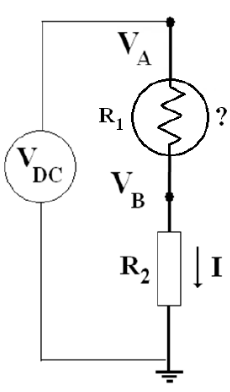
\includegraphics[width=.18\textwidth]{circuito_experimento}
  \caption{Circuito utilizado para verificação do fenômeno físico de mudança de resistência dependendo da temperatura.}
  \label{fig:circuito_experimento}
\end{figure}


\section{Resultados}

\subsection{Dados do experimento}


Os resultado capturados podem ser sumarizados na tabela \ref{tab:data_table}.


\begin{table*}[t]
\centering
\caption{Tabela com os dados coletados experimentalmente e os calculados em função dos dados coletados.}
\label{tab:data_table}
\begin{tabular}{|c|c|c|c|c|c|c|c|}
\hline
\textbf{$V_{DC}${[}V{]}} & \textbf{$V_A${[}V{]}} & \textbf{$V_B${[}V{]}} & \textbf{$V_{AB}${[}V{]}} & \textbf{I{[}A{]}} & \textbf{$R_1${[}$\Omega${]}} & \textbf{$P_1${[}W{]}} & \textbf{Cor}  \\ \hline
0                        & 0                     & 0                     & 0                        & 0                 & -                            & 0                     & -             \\ \hline
2                        & 2                     & 0,12                  & 1,88                     & 120 m             & 15,67                        & 225,60m               & VERMELHO      \\ \hline
4                        & 4                     & 0,15                  & 3,85                     & 150 m             & 25,67                        & 577,50m               & LARANJA       \\ \hline
6                        & 6                     & 0,19                  & 5,81                     & 190 m             & 30,58                        & 1,10                  & LARANJA       \\ \hline
8                        & 8                     & 0,21                  & 7,79                     & 210 m             & 37,09                        & 1,63                  & AMARELO       \\ \hline
10                       & 10                    & 0,23                  & 9,77                     & 230 m             & 42,47                        & 2,24                  & AMARELO CLARO \\ \hline
12                       & 12                    & 0,26                  & 11,74                    & 260 m             & 45,15                        & 3,05                  & AMARELO FORTE \\ \hline
\end{tabular}
\end{table*}

Em vias a comprovar a real captura dos dados, mostra-se as figuras \ref{fig:2V}, \ref{fig:4V}, \ref{fig:6V}, \ref{fig:8V}, \ref{fig:10V} e \ref{fig:12V}.

\begin{figure}[H]
  \centering
  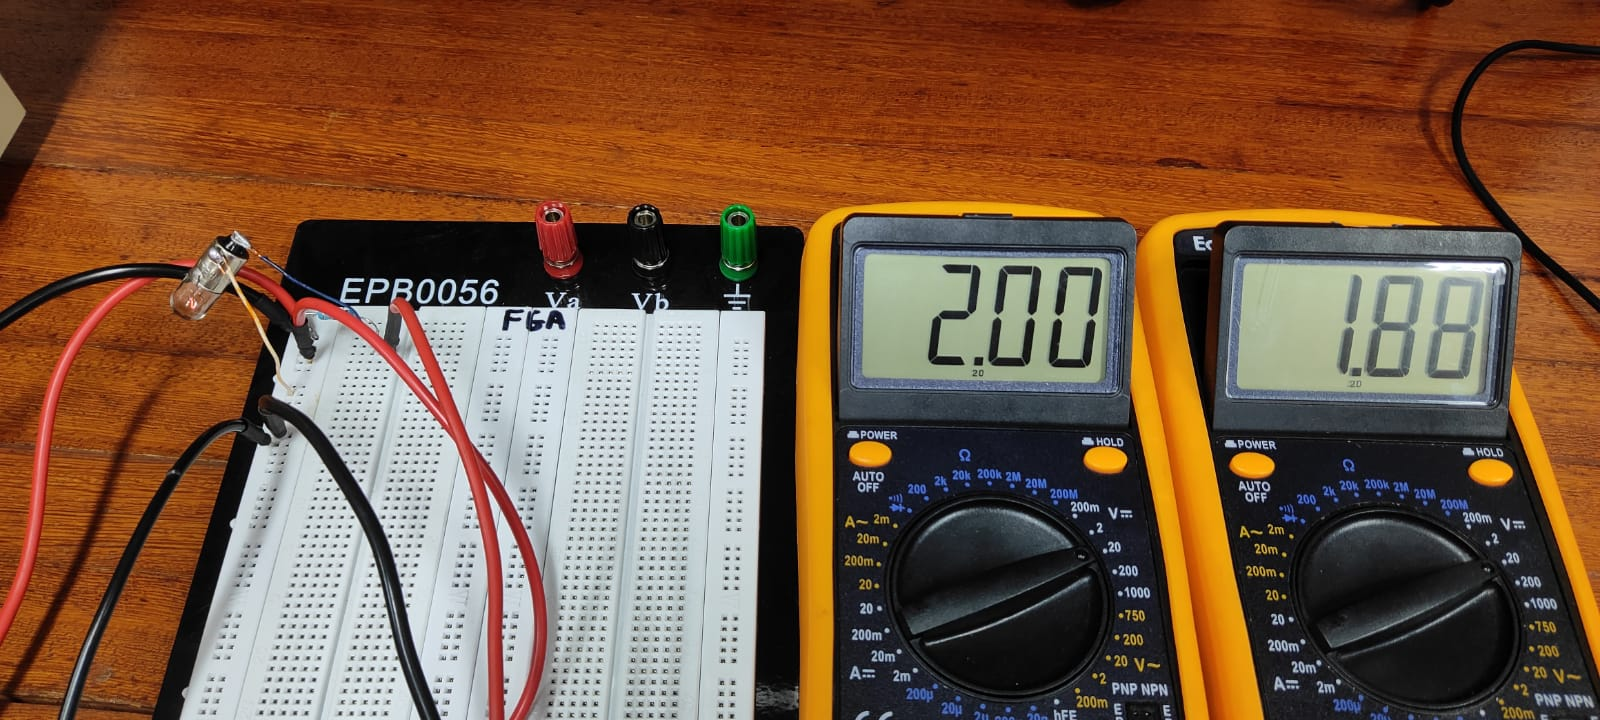
\includegraphics[width=.48\textwidth]{2V}
  \caption{Circuito com alimentação de 2V.}
  \label{fig:2V}
\end{figure}

\begin{figure}[H]
  \centering
  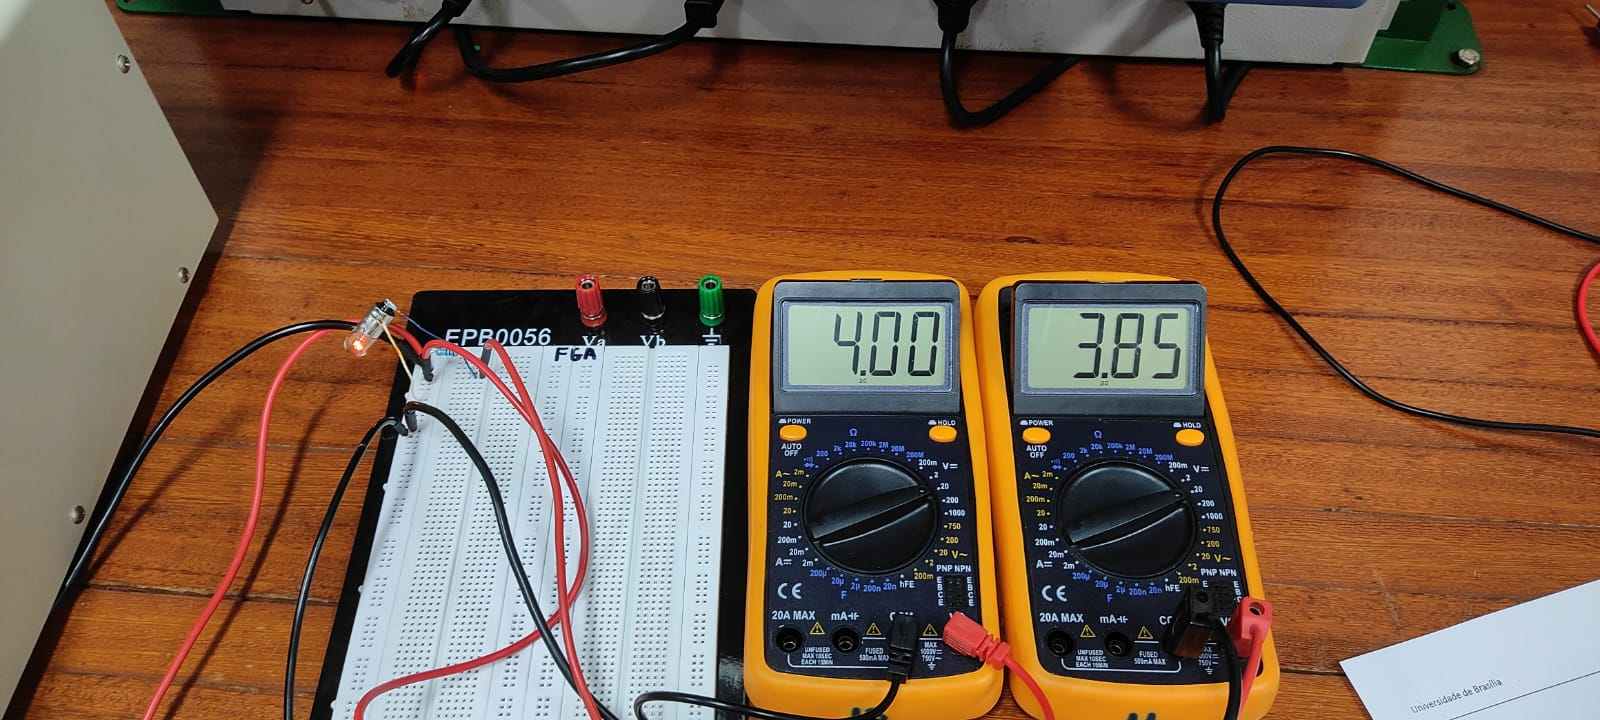
\includegraphics[width=.48\textwidth]{4V}
  \caption{Circuito com alimentação de 4V.}
  \label{fig:4V}
\end{figure}

\begin{figure}[H]
  \centering
  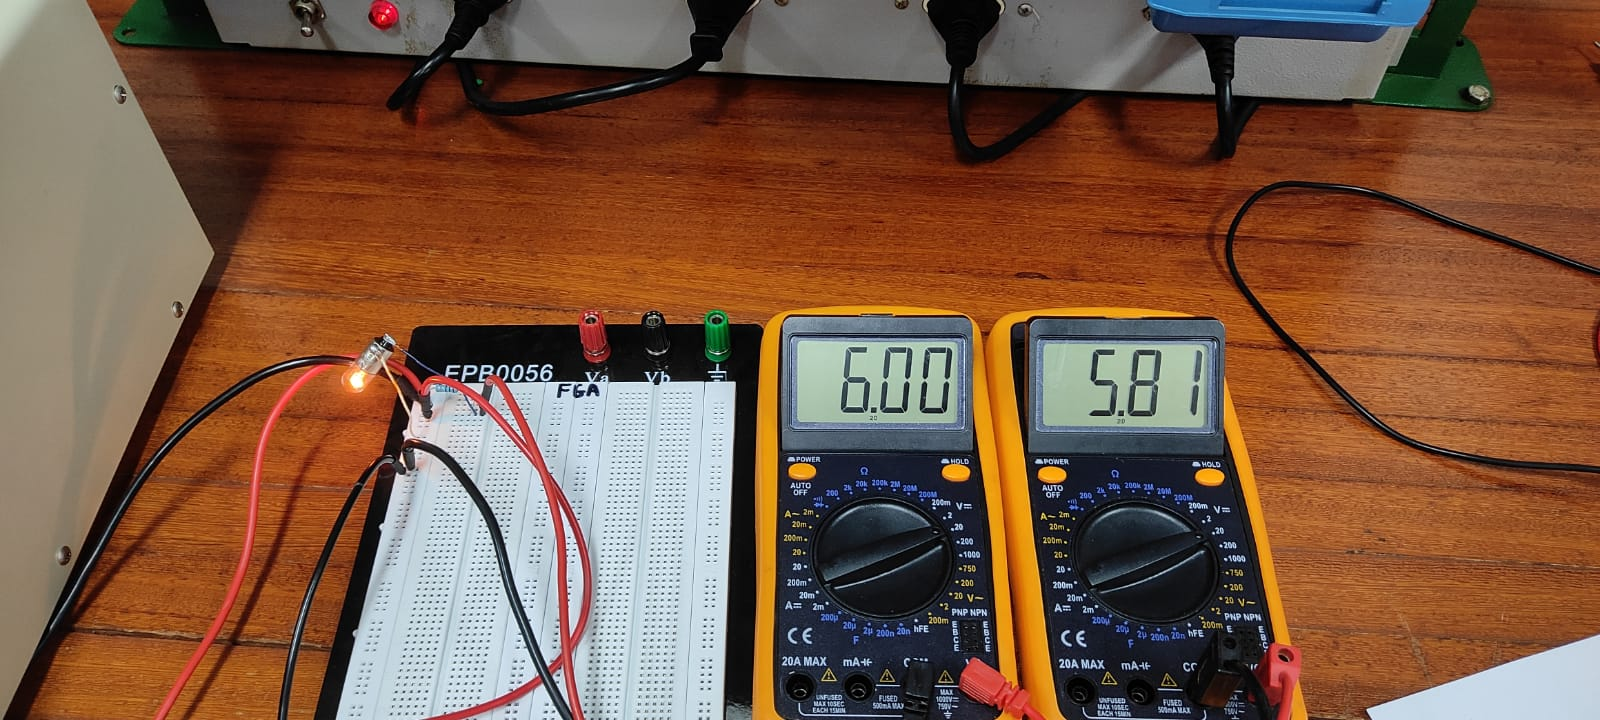
\includegraphics[width=.48\textwidth]{6V}
  \caption{Circuito com alimentação de 6V.}
  \label{fig:6V}
\end{figure}


\begin{figure}[H]
  \centering
  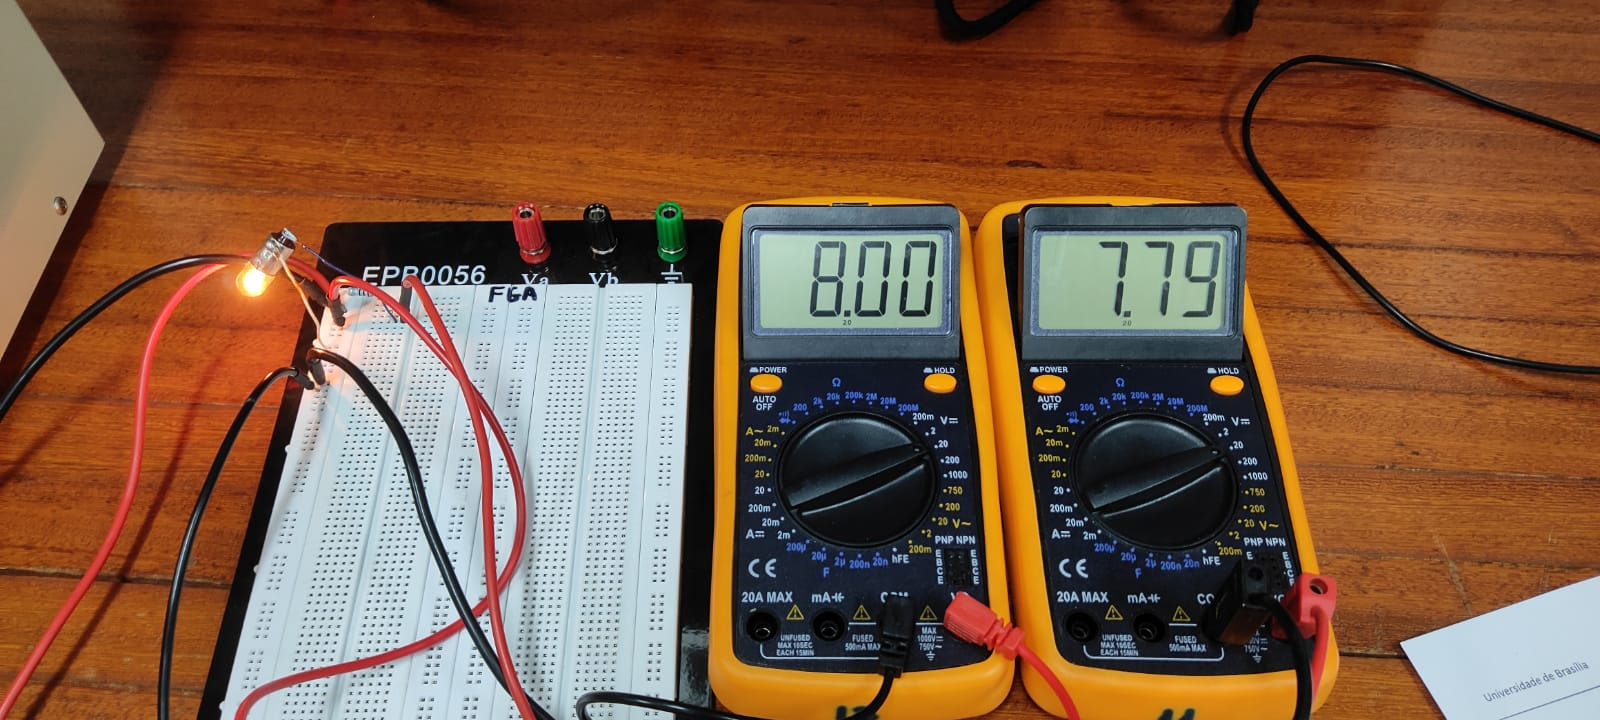
\includegraphics[width=.48\textwidth]{8V}
  \caption{Circuito com alimentação de 8V.}
  \label{fig:8V}
\end{figure}

\begin{figure}[H]
  \centering
  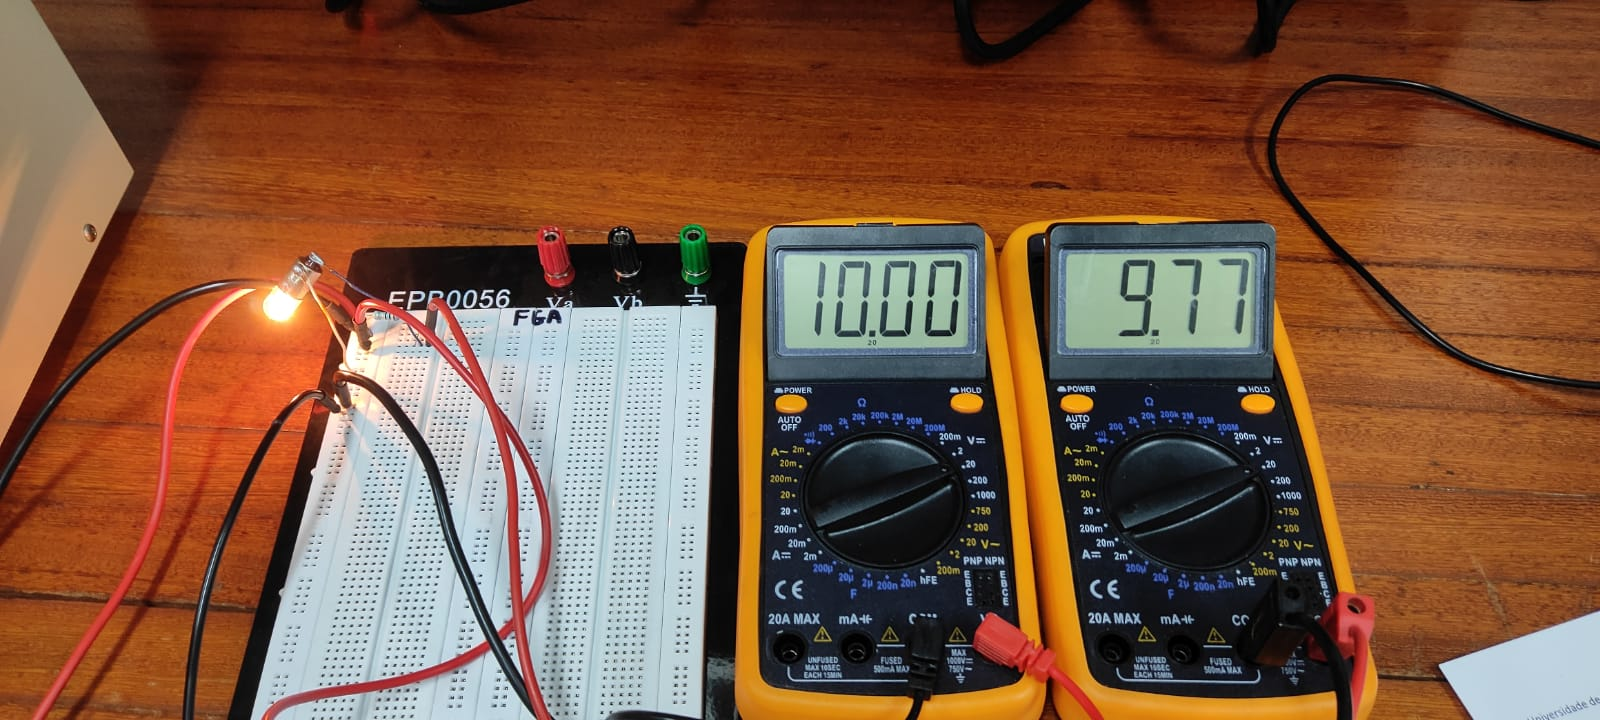
\includegraphics[width=.48\textwidth]{10V}
  \caption{Circuito com alimentação de 10V.}
  \label{fig:10V}
\end{figure}

\begin{figure}[H]
  \centering
  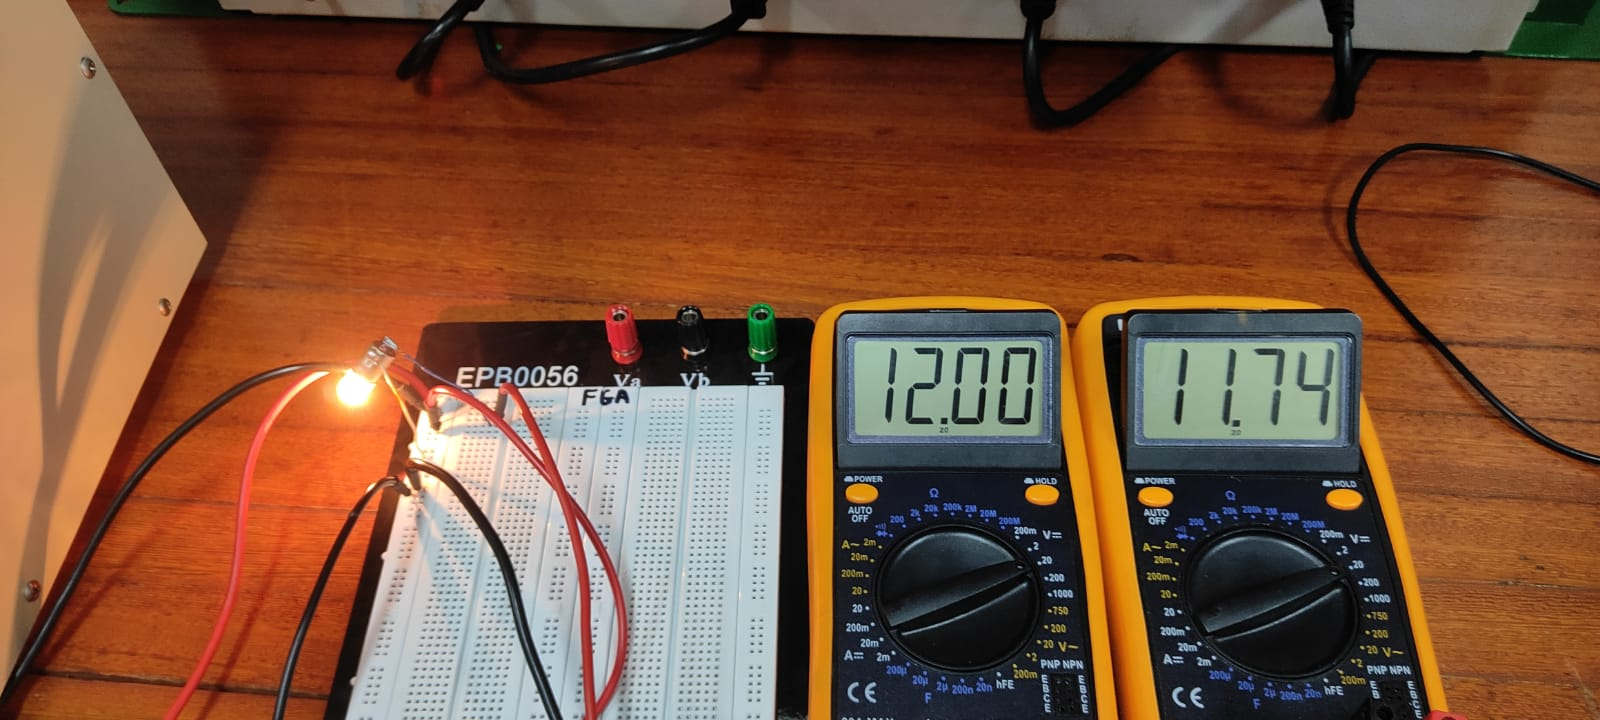
\includegraphics[width=.48\textwidth]{12V}
  \caption{Circuito com alimentação de 12V.}
  \label{fig:12V}
\end{figure}

Para montar o circuito, utilizamos um resistor R2 de $1\Omega$, com um erro médio de $5\%$. O real valor medido foi de $0,9\Omega$, o que condiz com o estabelecido como errático.

\subsection{Curva $I \times V_{AB}$ com a curva de correção}

\begin{figure}[H]
  \centering
  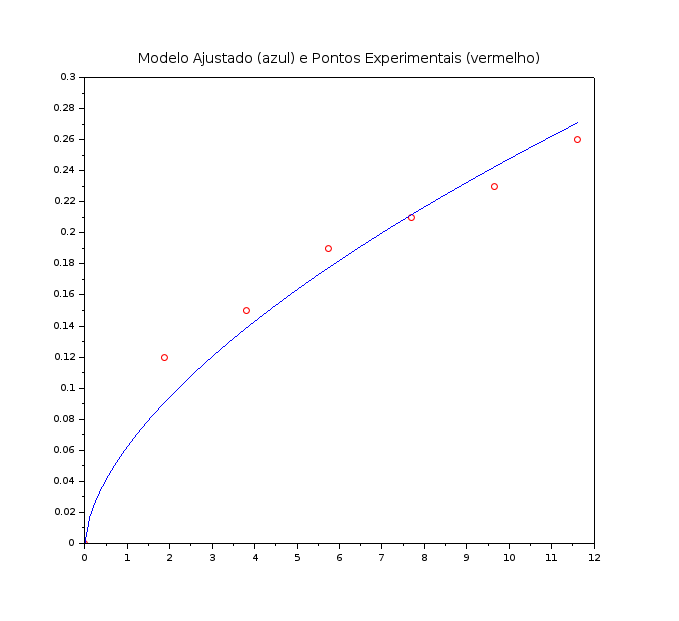
\includegraphics[width=.48\textwidth]{IXVAB}
  \caption{Curva de corrente (I) pela tensão sobre a lâmpada ($V_{AB}$).}
  \label{fig:IXVAB}
\end{figure}

O valor do erro quadrátivo médio é de 0.0002036, o que constituí um modelo adequado para os pontos experimentais obtidos. Logo, pode-se concluir que houve sucesso na realização do experimento.

\section{Questionário}

\subsection{Assumindo um espectro de radiação de corpo negro para o Sol, estabeleça o comprimento de onda de máxima radiação ($\lambda_{max}$), sabendo que a temperatura da superfície é de 5800 [K]. Qual o percentual da potência irradiada na forma de fótons com comprimento de onda menor que $\lambda_{max}$.}

Para tal temperatura temos o comprimento de onda de aproximadamente $545 nm$. A potência irradiada pelo sol é vista na equação \ref{eq:pot_sol}.

\begin{gather}\label{eq:pot_sol}
  P_R = A\epsilon \sigma T^4 = 3.90\times 10^{20} W
\end{gather}


\subsection{Um bom modelo permite prever o comportamento de uma lâmpada em pontos experimentais nunca medidos. Usando o modelo ajustado, calcule o valor da resistência de equilíbrio $R_1$, para a tensão negativa $V_{AB}=-5,0V$. Apresente a memória de cálculo do valor de $R_1$ e justifique a sua validade.}


Para prever o compartamento da lâmpada, temos que realizar a construção por meio de um ajuste não linear. Como visto na aula, o modelo a ser utilizado pode ser visto na equação \ref{eq:aprox}.

\begin{gather}\label{eq:aprox}
  I \simeq KV^{\dfrac{3}{5} }
\end{gather}

Com os dados obtidos anteriormente, já temos a constante K já calculada, e a partir dela podemos encontar o valor de -5V. Dado que está elevado a uma potência fracionária, o resultado será imaginário, e com isso será necessário tirar o valor absoluto de tal valor. Assim, tem-se o valor calculado visto na equação \ref{eq:current}.

\begin{gather}\label{eq:current}
  |I| \simeq  0.1634027 [A]
\end{gather}


\end{document}
